
\begin{frame}\frametitle{Physics objects puzzle}
\centering\myskip

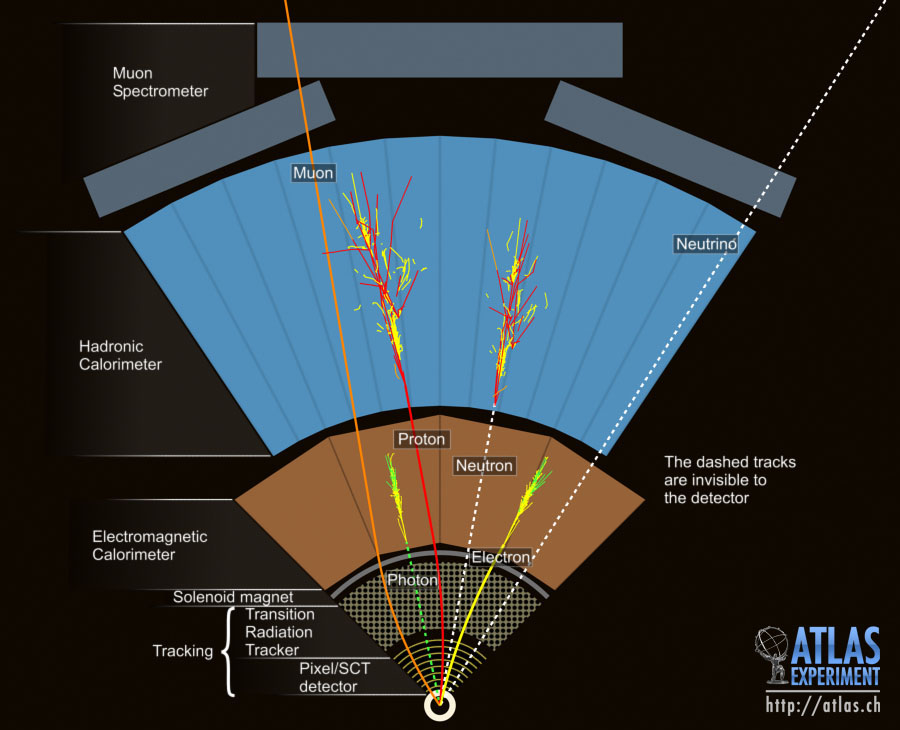
\includegraphics[height=0.85\textheight, width=1.\textwidth]{../detector/figures/detection}

\end{frame}



\begin{frame}\frametitle{One lepton}
\footnotesize\centering

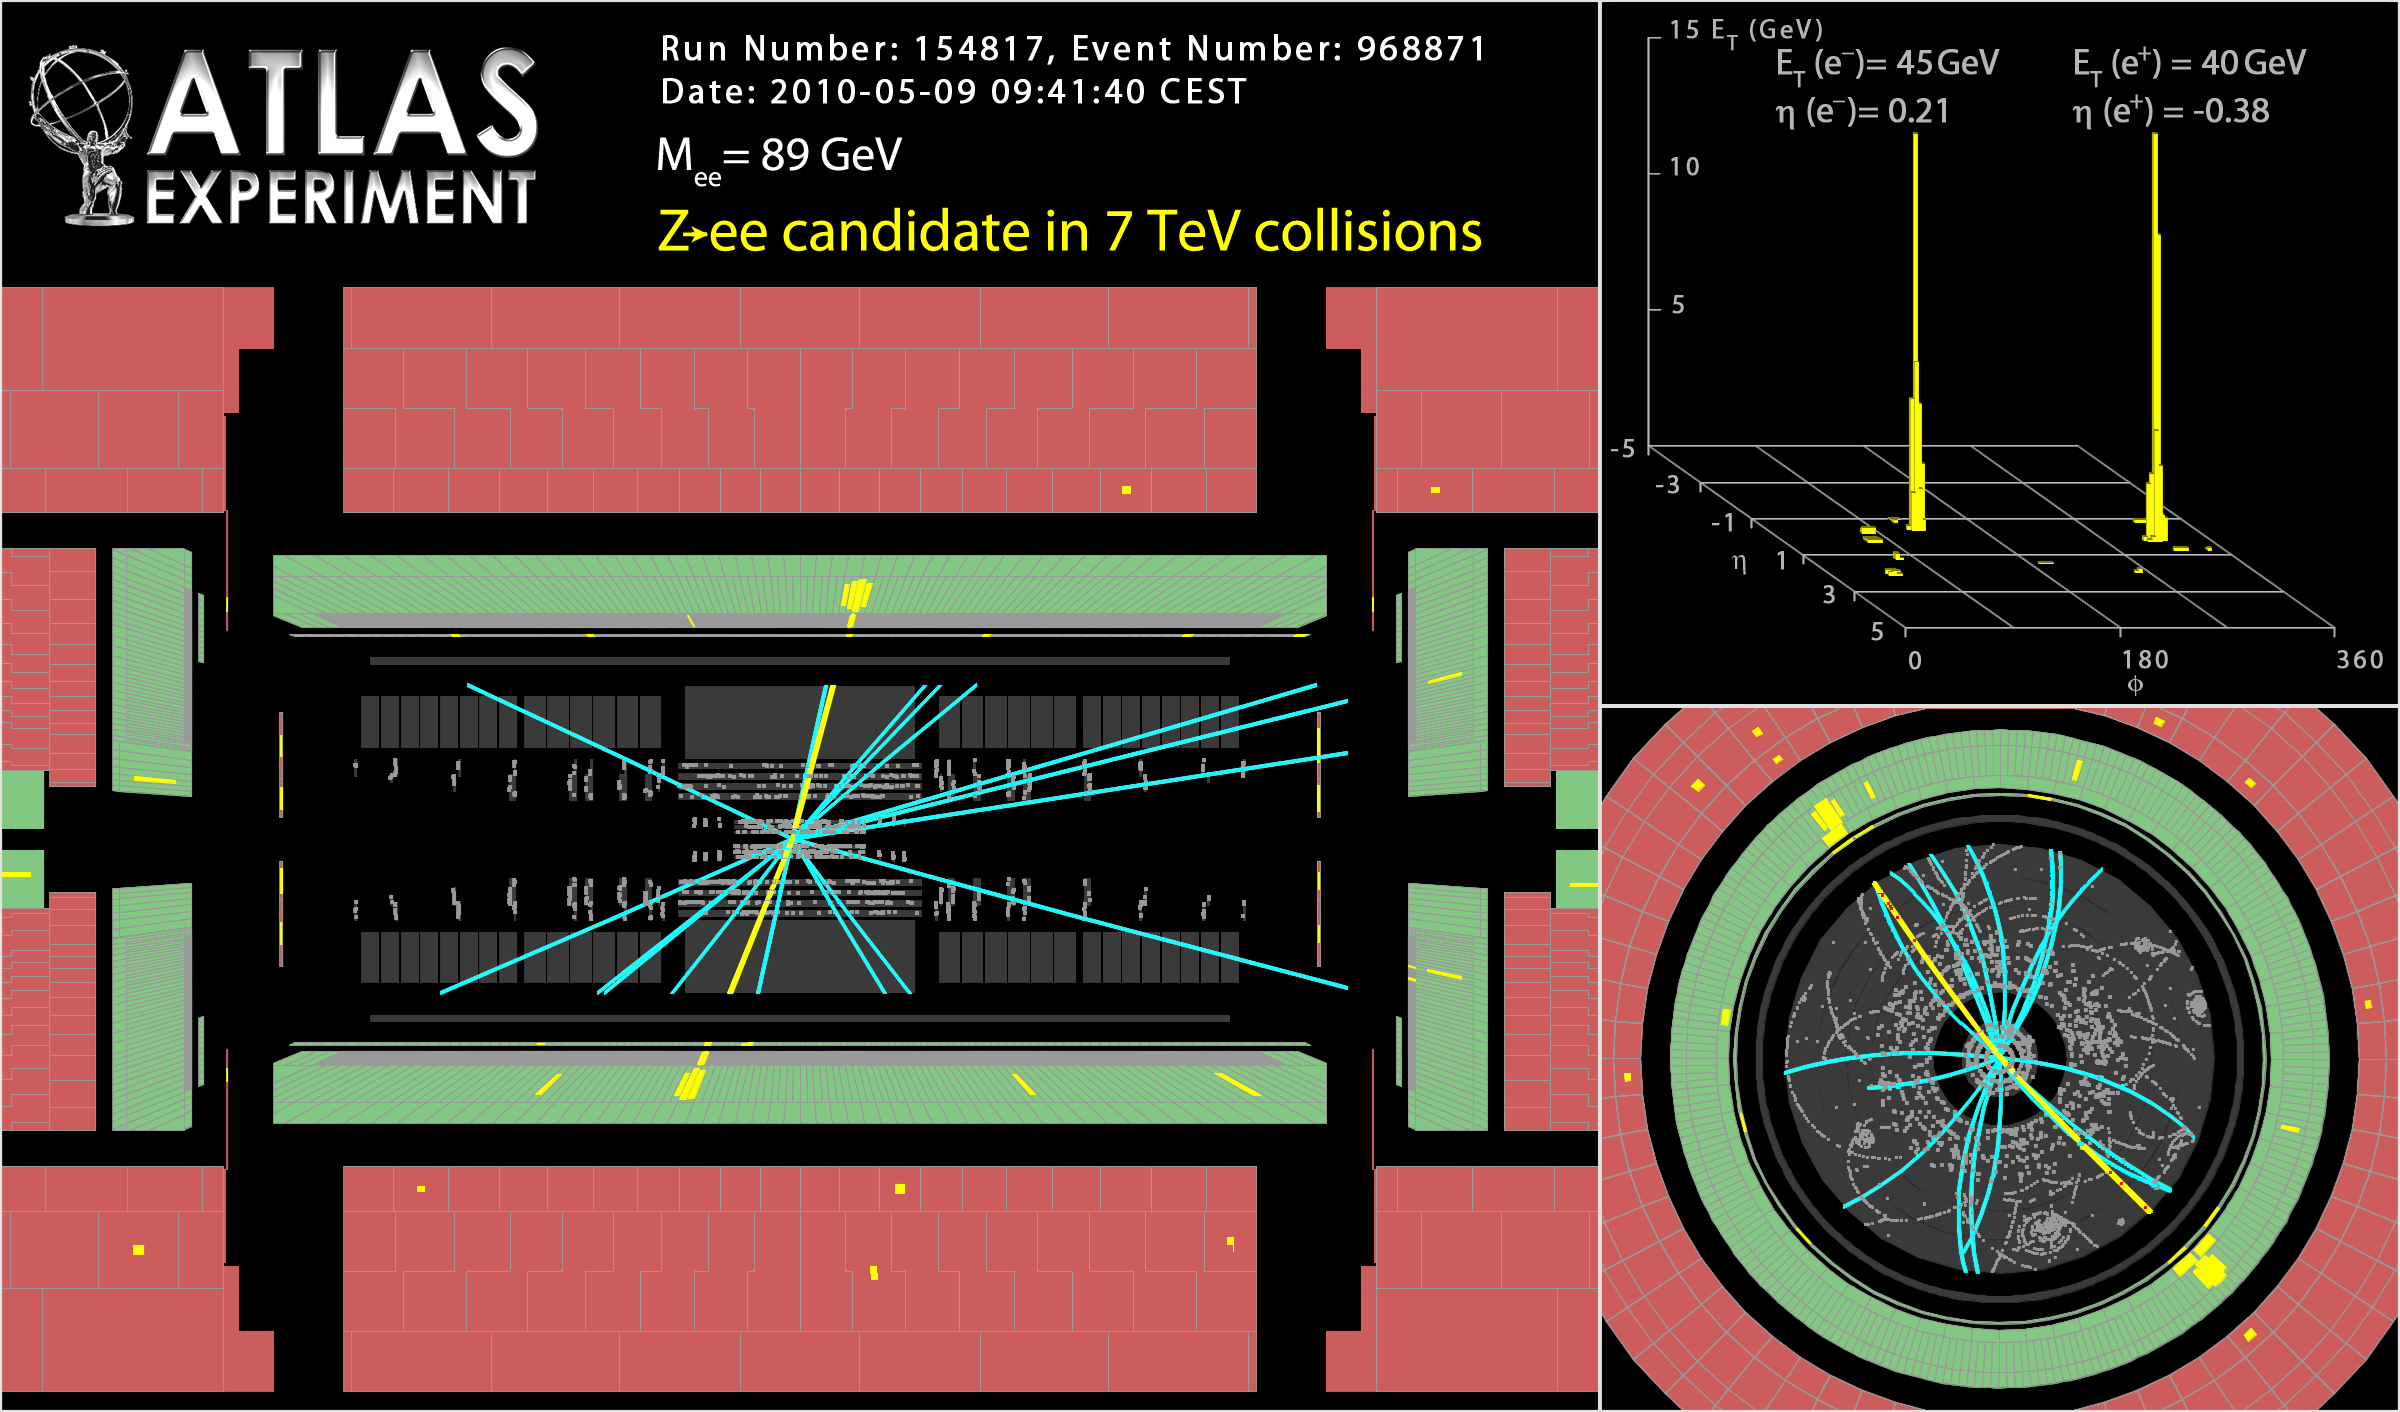
\includegraphics[width=.5\textwidth,height=0.5\textheight]{pics/Zee}
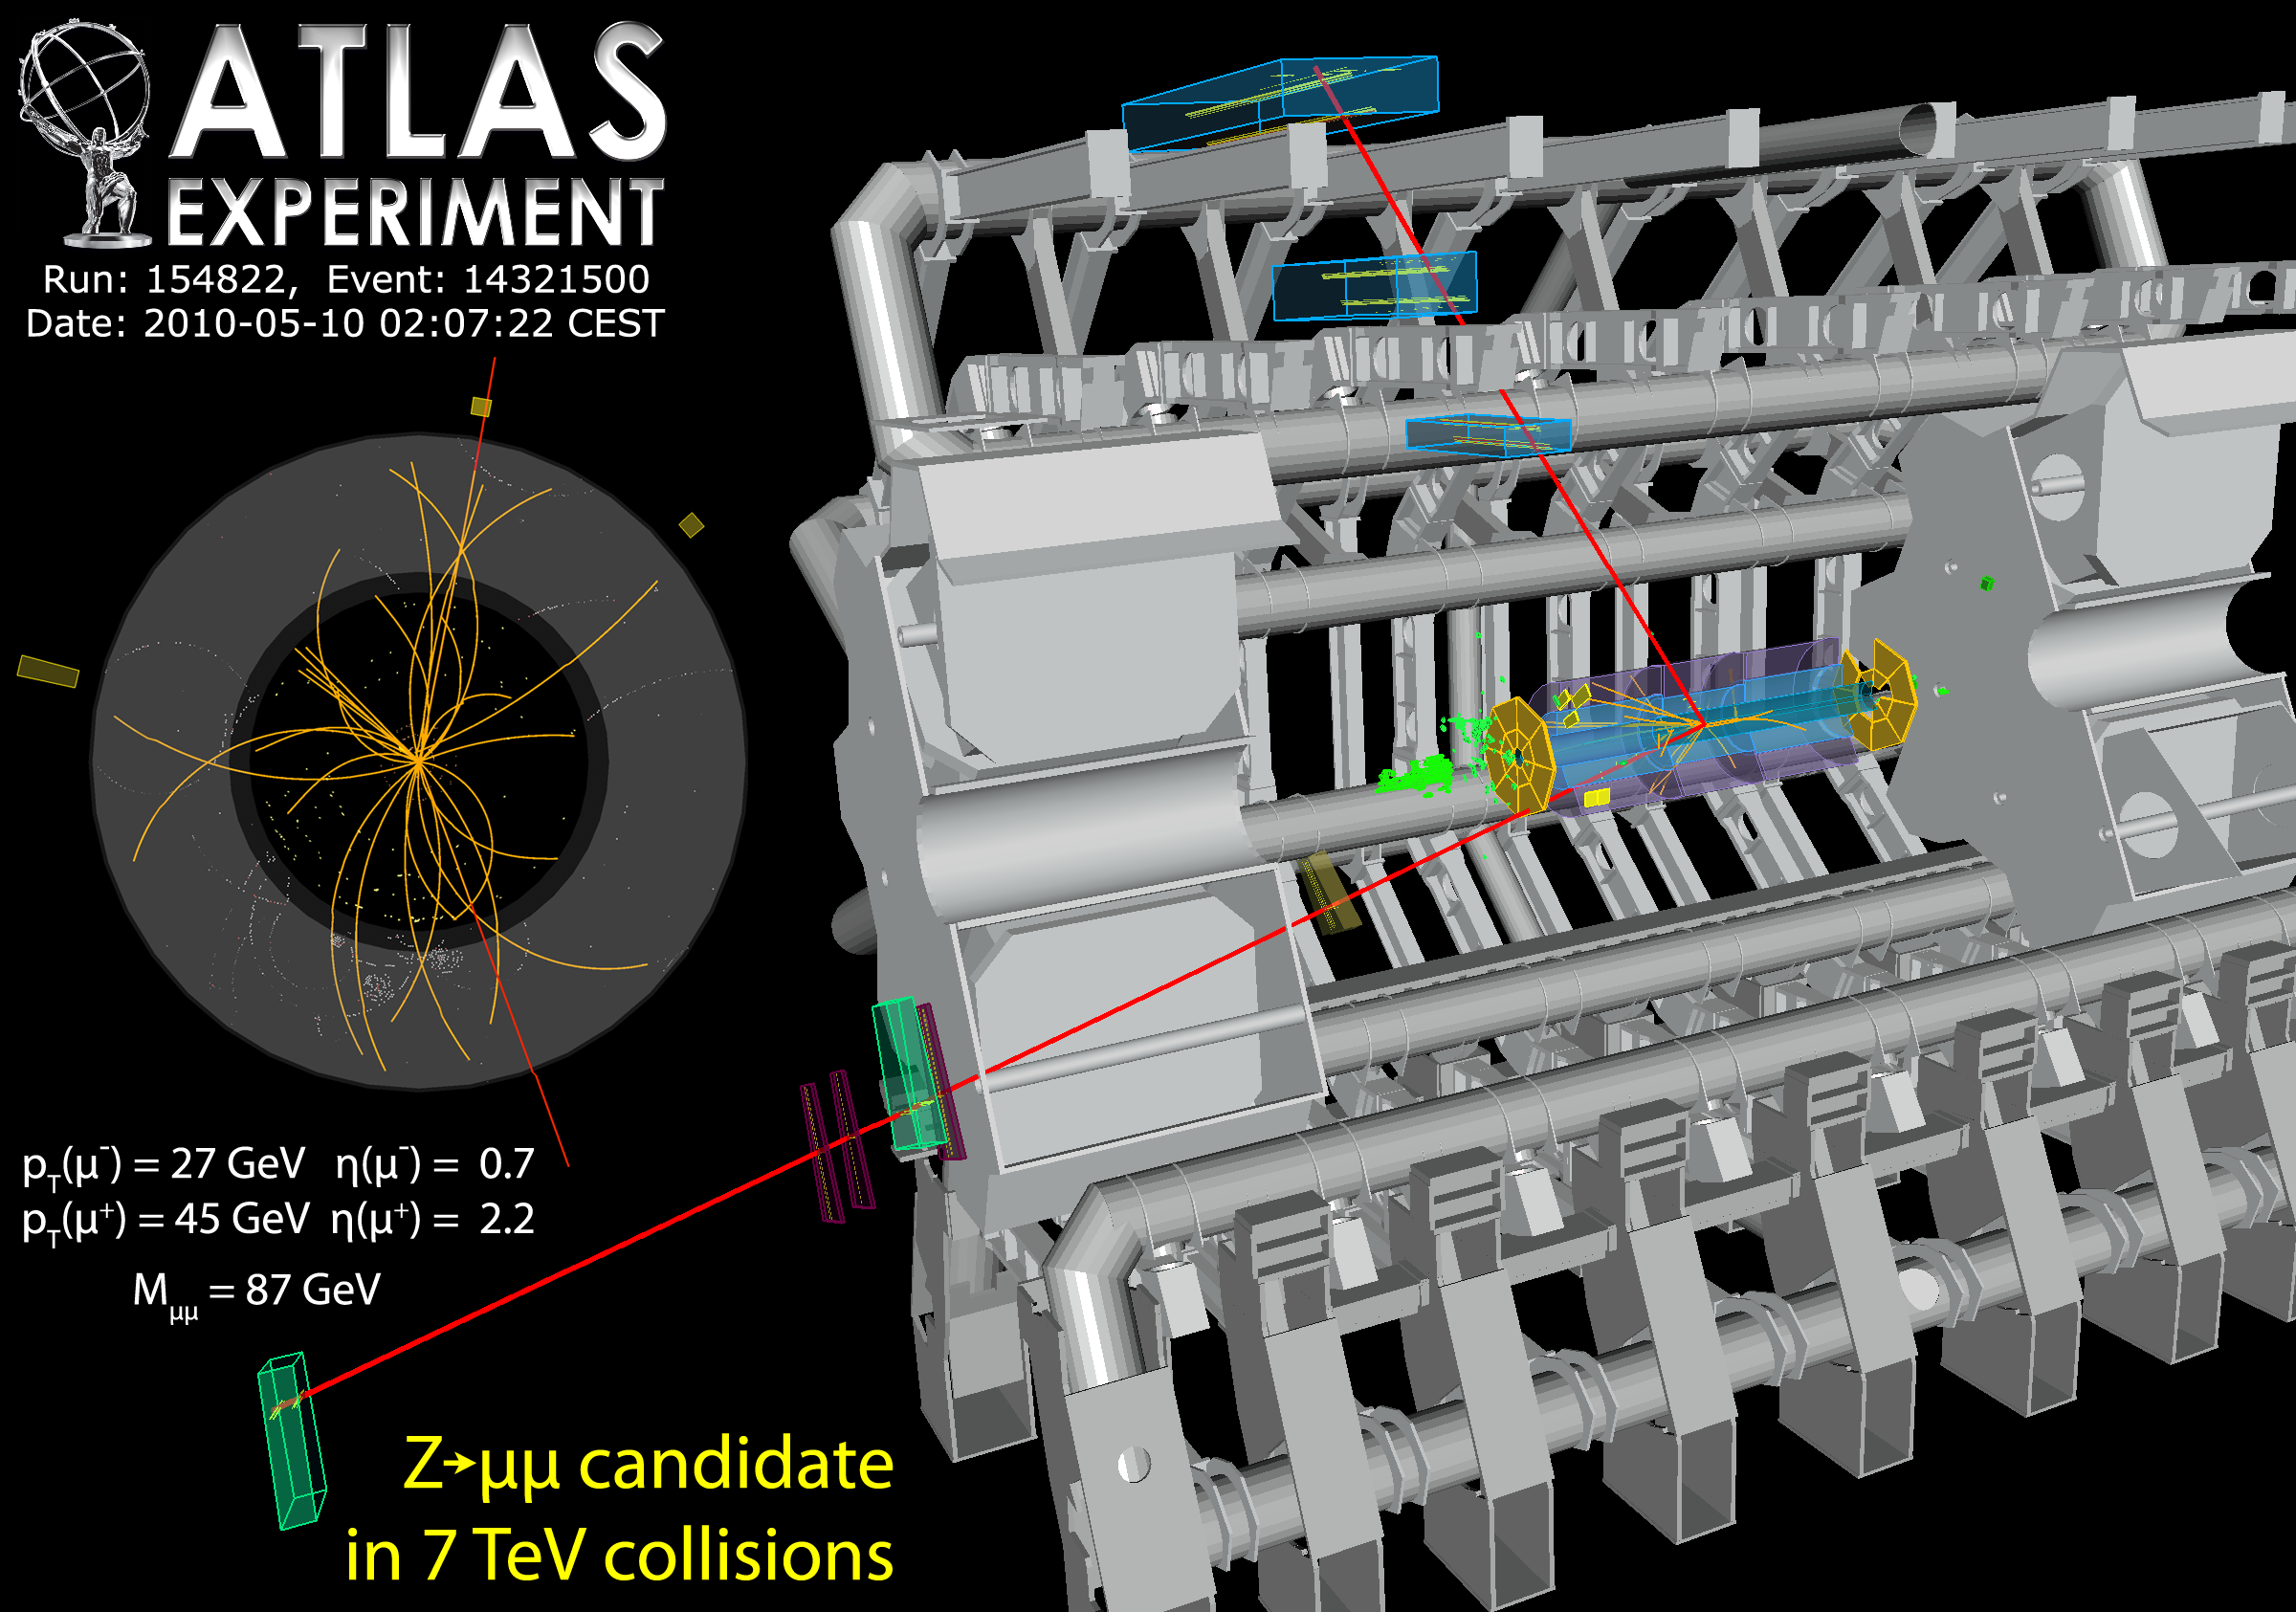
\includegraphics[width=.5\textwidth,height=0.5\textheight]{pics/Zmumu}

\begin{minipage}{.5\textwidth}\centering

\begin{itemize}
\item $|\eta|<2.5$ ID track $\leftrightarrow$ EM deposit
\end{itemize}

\end{minipage}\begin{minipage}{.5\textwidth}\centering

\begin{itemize}
\item \texttt{Muid}: MS track $\leftrightarrow$ ID track ($|\eta|<2.5$)
\end{itemize}

\end{minipage}

\begin{minipage}{.5\textwidth}\centering

\begin{itemize}
\item calibrated with $Z\to ee (\mu\mu)$ events
\end{itemize}
{\cccolor \bfseries \large +}\\
\begin{itemize}
\item isolated
\item $\pt (\et) > 25\gev$, $|z_0|<2~$mm
\item match to the lepton triggering the event
\end{itemize}
\end{minipage}

\end{frame}



\begin{frame}\frametitle{Many jets}
\centering\footnotesize

\begin{minipage}{.5\textwidth}\centering

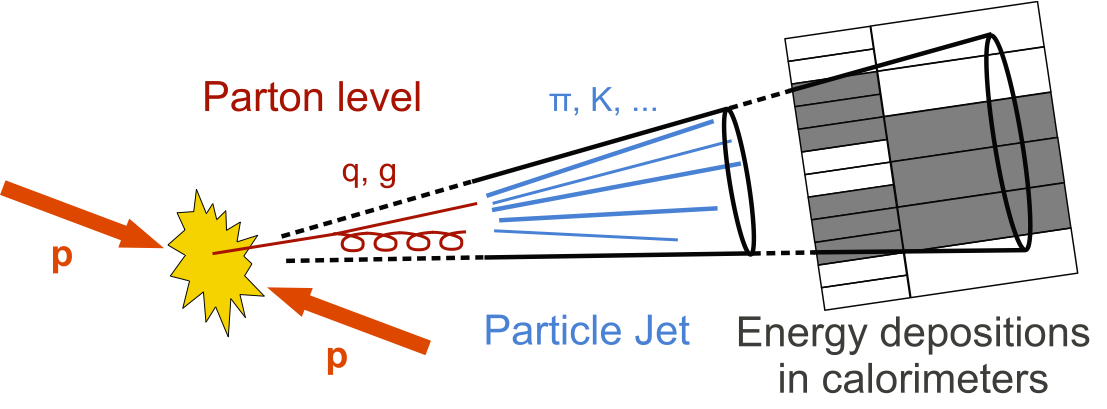
\includegraphics[width=.78\textwidth]{pics/Sketch_PartonParticleCaloJet.png}\\
%\resizebox{1.\textwidth}{!}{from \url{http://cms.web.cern.ch/news/jets-cms-and-determination-their-energy-scale}}

\begin{itemize}
\item Combine calorimeter clusters using anti-$k_t$ algorithm with $R=0.4$
\end{itemize}
$d_{ij}=min(\dfrac{1}{k_{t_i}^{2}},\dfrac{1}{k_{t_j}^{2}})\frac{\Delta R_{ij}^{2}}{R^{2}}$
\begin{itemize}
\item LocalCluster calibration of energy
\item Pile-up and particle-level $E$ corrections
\end{itemize}
{\cccolor \bfseries +}\\
\begin{itemize}
\item $\pt>25\gev$, $|\eta|<2.5$
\item coming from primary vertex
\end{itemize}


\end{minipage}\begin{minipage}{.5\textwidth}\centering

\vskip-5ex
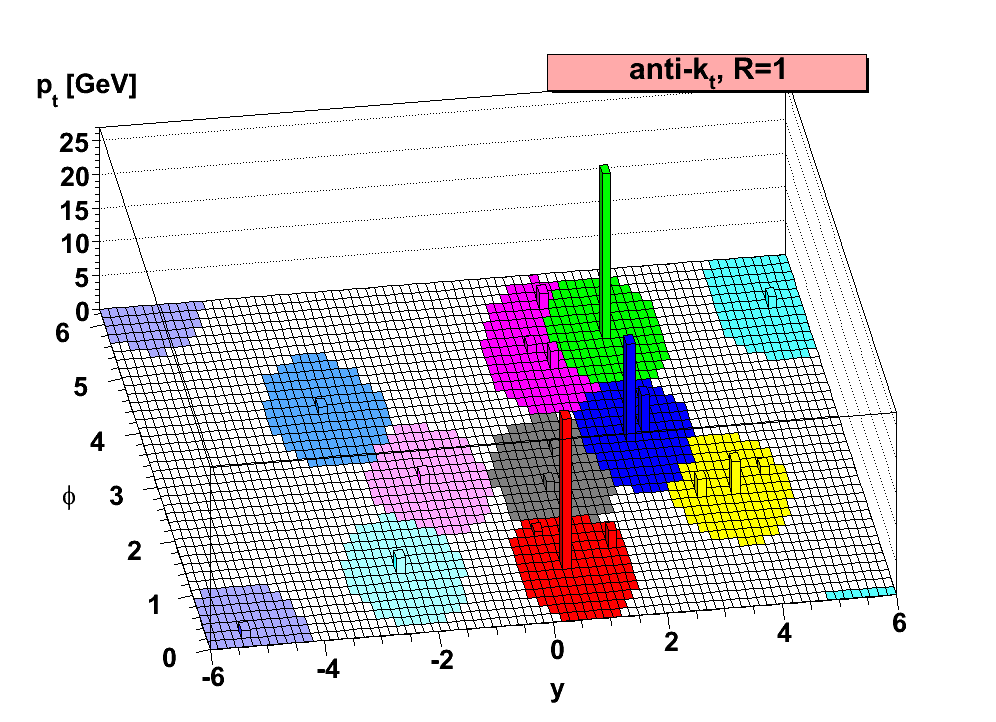
\includegraphics[width=.8\textwidth]{pics/antikt}\\
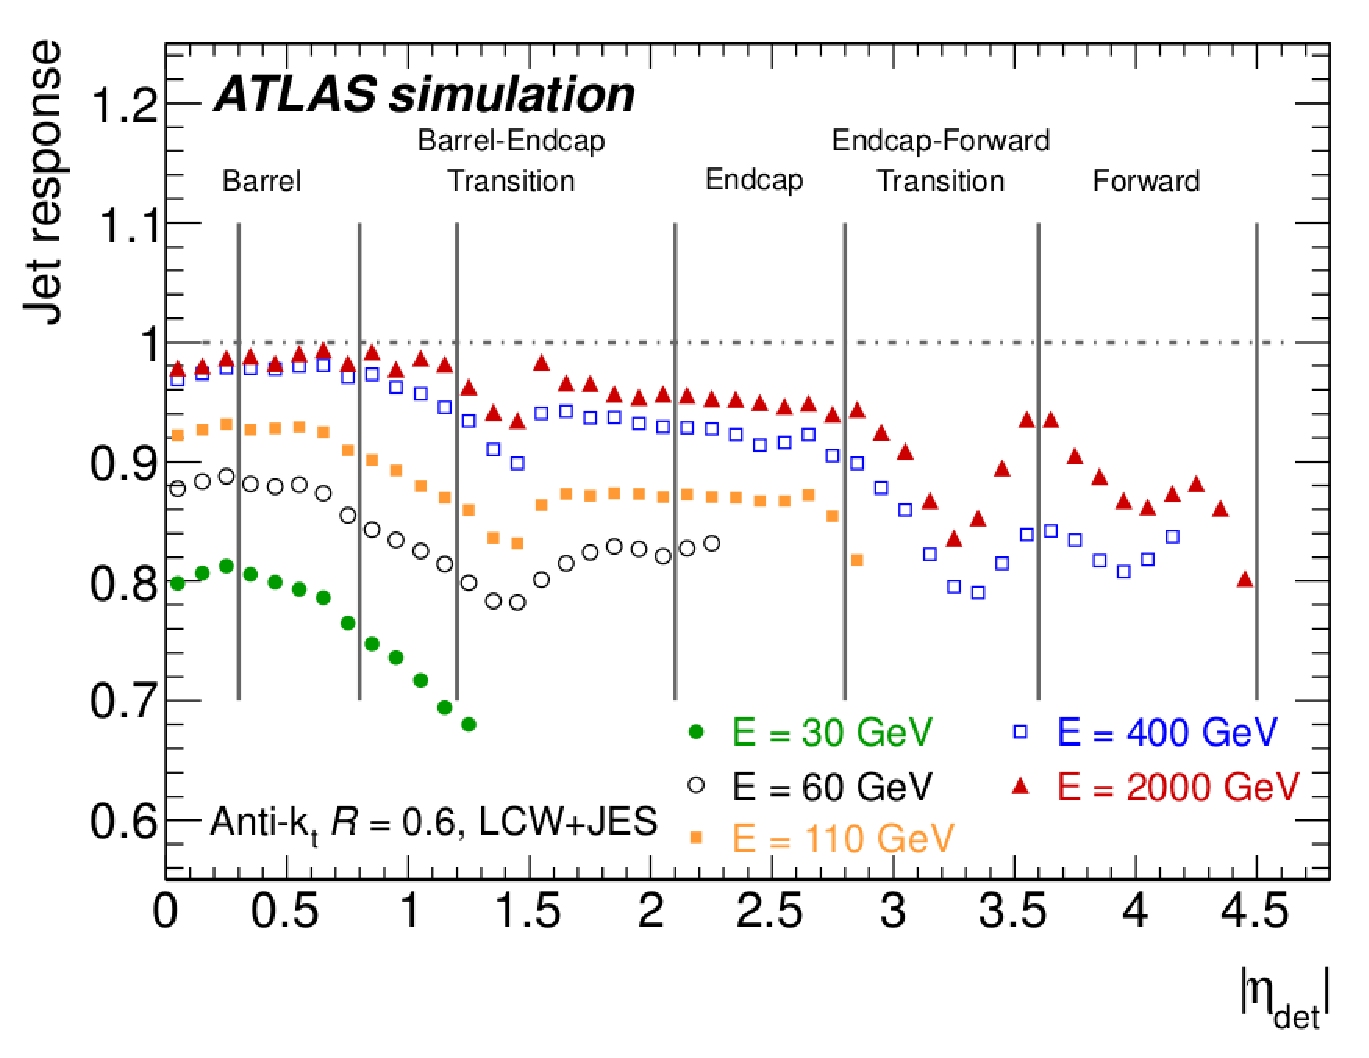
\includegraphics[width=.9\textwidth]{pics/corr_jet_lcw}

\end{minipage}


\end{frame}



\begin{frame}\frametitle{\btag ging}
\centering\footnotesize

\begin{minipage}{.5\textwidth}\centering

$b$ quark $\Rightarrow$ $B$ hadron ($\lambda\sim 10^{-12}$~s)\\
{\large$\Downarrow$}\\
travels about 3~mm before decaying

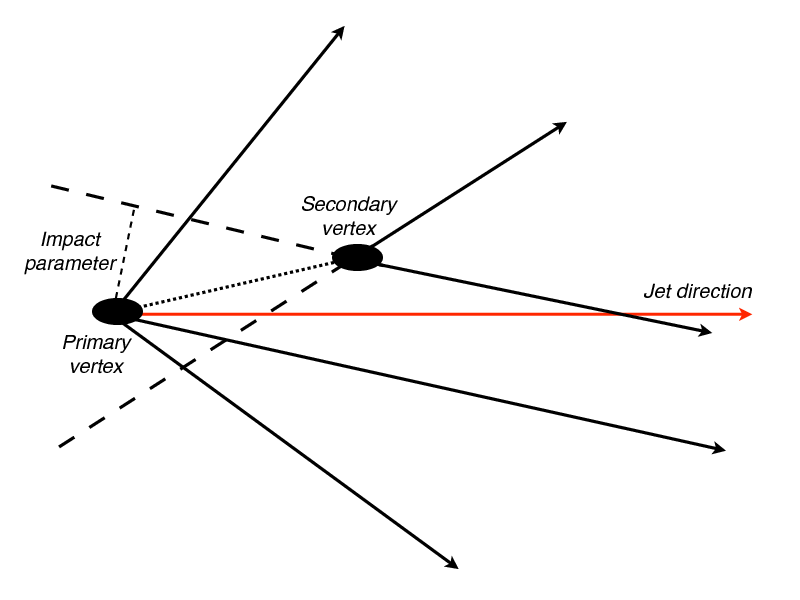
\includegraphics[width=.5\textwidth]{../objectsreconstruction/figures/Picture-b-tagging-2.png}

\end{minipage}\begin{minipage}{.5\textwidth}\centering

\includegraphics[width=.8\textwidth]{pics/blighteff}

\end{minipage}

\myskip


multi-variate algorithm combining info from {\cccolor impact parameters}\\
and the {\cccolor reconstructed secondary vertex} 

\begin{itemize}
\item 70\% efficiency, $\sim 130$ light-jet rejection, $\sim 5$ $c$-jet rejection
\end{itemize}

\end{frame}



\begin{frame}\frametitle{Missing transverse energy}
\centering\myskip


\begin{minipage}{.6\textwidth}\centering
\includegraphics[width=.9\textwidth]{pics/MET-photon-ATLAS.jpg}\\

\end{minipage}\begin{minipage}{.4\textwidth}\centering

Invisible particles\\
{\footnotesize (neutrinos and\dots who knows!)}\\
{\Large$\Downarrow$}\\
Quantify the $E$ imbalance in the transverse plane

\end{minipage}

$$\begin{array}{lcl}
%E^{\rm miss}_{x,y} & = & E^{\rm RefEle}_{x,y} + E^{\rm RefGamma}_{x,y} + E^{\rm RefJet}_{x,y} + E^{\rm RefMuon}_{x,y} + E^{\rm SoftJet}_{x,y} + E^{\rm CellOut}_{x,y}\\
E^{\rm miss}_{T} & = & \big|-\sum\vec{p}_T \big| = \sqrt{(E^{\rm miss}_{x})^2 + (E^{\rm miss}_{y})^2} ,\\
E^{\rm miss}_{x} & = & -\sum\vec{p}_x ,\\
E^{\rm miss}_{y} & = & -\sum\vec{p}_y ,\\
\end{array}$$



\end{frame}

